\documentclass{beamer}
%\usepackage[margin=1in]{geometry}
\usepackage{amsthm,amsmath,amsfonts,hyperref,graphicx,color,multicol}
\usepackage{enumitem,tikz}
\usepackage{booktabs}
%%%%%%%%%%
%Beamer Template Customization
%%%%%%%%%%
\setbeamertemplate{navigation symbols}{}
\setbeamertemplate{theorems}[ams style]
\setbeamertemplate{blocks}[rounded]

\definecolor{Blu}{RGB}{43,62,133} % UWEC Blue
\setbeamercolor{structure}{fg=Blu} % Titles

%Unnumbered footnotes:
\newcommand{\blfootnote}[1]{%
	\begingroup
	\renewcommand\thefootnote{}\footnote{#1}%
	\addtocounter{footnote}{-1}%
	\endgroup
}


%%%%%%%%%%
%Custom Commands
%%%%%%%%%%
\newcommand{\R}{\mathbb{R}}
\newcommand{\veca}{\vec{a}}
\newcommand{\vecb}{\vec{b}}
\newcommand{\vece}{\vec{e}}
\newcommand{\vecu}{\vec{u}}
\newcommand{\vecv}{\vec{v}}
\newcommand{\vecw}{\vec{w}}
\newcommand{\vecx}{\vec{x}}
\newcommand{\zerovector}{\vec{0}}

\newcommand{\ds}{\displaystyle}

\newcommand{\fn}{\insertframenumber}

\newcommand{\col}{\operatorname{col}}
\newcommand{\row}{\operatorname{row}}
\newcommand{\rank}{\operatorname{rank}}
\newcommand{\nullity}{\operatorname{nullity}}
\newcommand{\adj}{\operatorname{adj}}
\newcommand{\proj}{\operatorname{proj}}
\newcommand{\ip}[2]{\left\langle #1,#2\right\rangle}

\newcommand{\blank}[1]{\underline{\hspace*{#1}}}

\newcommand{\dotp}{\,{\boldsymbol{\cdot}\hspace*{.01in}}}

%%%%%%%%%%
%Custom Theorem Environments
%%%%%%%%%%
\theoremstyle{definition}
\newtheorem{exercise}{Exercise}
\newtheorem{question}[exercise]{Question}
\newtheorem*{defn}{Definition}
\newtheorem*{exa}{Example}
\newtheorem*{disc}{Group Discussion}
\newtheorem*{nb}{Note}
\newtheorem*{recall}{Recall}
\renewcommand{\emph}[1]{{\color{blue}\texttt{#1}}}

\definecolor{Gold}{RGB}{237, 172, 26}
%Statement block
\newenvironment{statementblock}[1]{%
	\setbeamercolor{block body}{bg=Gold!20}
	\setbeamercolor{block title}{bg=Gold}
	\begin{block}{\textbf{#1.}}}{\end{block}}





\begin{document}
	\title{Math 324: Linear Algebra}
	\subtitle{Section 6.3: Matrices for Linear Transformations}
	\author{Mckenzie West}
	\date{Last Updated: \today}
\begin{frame}[fragile]
\maketitle	
\end{frame}

\begin{frame}{\insertframenumber}
	\begin{block}{\textbf{Last Time.}}
	\begin{itemize}[label=--]
		\item One-to-One Transformations
		\item Onto Transformations
		\item Isomorphisms
	\end{itemize}
	\end{block}
	\begin{block}{\textbf{Today.}}
		\begin{itemize}[label=--]
			\item The matrix of a transformation.
			\item Compositions
		\end{itemize}
	\end{block}
\end{frame}
\begin{frame}{\fn}
	\begin{recall}
		Linear transformations can be defined by their action on a basis.
	\end{recall}
	\begin{exercise}
		Suppose $T:\R^2\to\R^3$ satisfies $T(1,0)=(3,2,1)$ and $T(0,1)=(1,1,1)$.
		
		What is $T(3,-8)$?
	\end{exercise}
\end{frame}
\begin{frame}{\fn}\mbox{}\vskip-.5in
	\begin{statementblock}{Theorem 6.10}
		Let $T\colon \R^n\to \R^m$ be a linear transformation such that, for the standard basis vectors $\vec e_i$ of $\R^n$,
			\[T(\vec e_1)=\begin{bmatrix}a_{11}\\a_{21}\\\vdots\\a_{m1}	\end{bmatrix},\ 
			T(\vec e_2)=\begin{bmatrix}a_{12}\\a_{22}\\\vdots\\a_{m2}\end{bmatrix},\ \dots,
			T(\vec e_n)=\begin{bmatrix}a_{1n}\\a_{2n}\\\vdots\\a_{mn}\end{bmatrix}.
			\]
		Then the $m\times n$ matrix whose $n$ columns correspond to $T(\vec e_i)$,
			\[A=\begin{bmatrix}
				a_{11}&a_{12}&\cdots&a_{1n}\\
				a_{21}&a_{22}&\cdots&a_{2n}\\
				\vdots&\vdots&&\vdots\\
				a_{m1}&a_{m2}&\cdots&a_{mn}
				\end{bmatrix}\]
		satisfies $T(\vec v)=A\vec v$ for every $\vec v\in\R^n$.  We call $A$ the \emph{standard matrix} for $T$.
	\end{statementblock}
\end{frame}
\begin{frame}{\fn}
	\begin{exercise}
		Consider the transformation from exercise 1, $T:\R^2\to\R^3$ such that $T(1,0)=(3,2,1)$ and $T(0,1)=(1,1,1)$.
		\begin{enumerate}[label=(\alph*)]
			\item 
			Find the standard matrix for $T$.
			\item
			Use the standard matrix to compute $T(-2,6)$.
		\end{enumerate}
	\end{exercise}
	\begin{exercise}
		Find the standard matrix for $T\colon \R^3\to\R^2$ defined by $T(x,y,z)=(2x+y,2x-z)$.
	\end{exercise}
	\begin{exercise}[Optional]
		Consider the transformation $T\colon \R^2\to\R^2$ that is given by rotation 60$^\circ$ counterclockwise. Find the standard matrix for $T$ using a little trigonometry and the action of this transformation on the basis vectors $\vec e_1=(1,0)$ and $\vec e_2=(0,1)$.
	\end{exercise}
\end{frame}
%\begin{frame}{\fn}
%	\begin{exercise}
%		Consider the transformation $T\colon P_2\to P_2$ defined by $T(ax^2+bx+c)=ax^2+(a+b)x+(a+b+c)$.
%		We can view each polynomial $p(x)=ax^2+bx+c$ as a vector in $\R^3$ by associating it with the vector $[p]=\begin{bmatrix}a\\b\\c\end{bmatrix}$.  Now proceed to find the standard matrix for $T$ with respect to this association to $\R^3$.
%	\end{exercise}
%\end{frame}
\begin{frame}{\fn}
	\begin{defn}
		The \emph{composition} of the transformations $T_1\colon \R^n\to \R^m$ with $T_2\colon \R^m\to\R^k$ is the transformation $T\colon \R^n\to\R^k$ defined by 
			\[T(\vec v)=T_2(T_1(\vec v)).\]
		Denote the composition by $T=T_2\circ T_1$.
		\begin{center}
			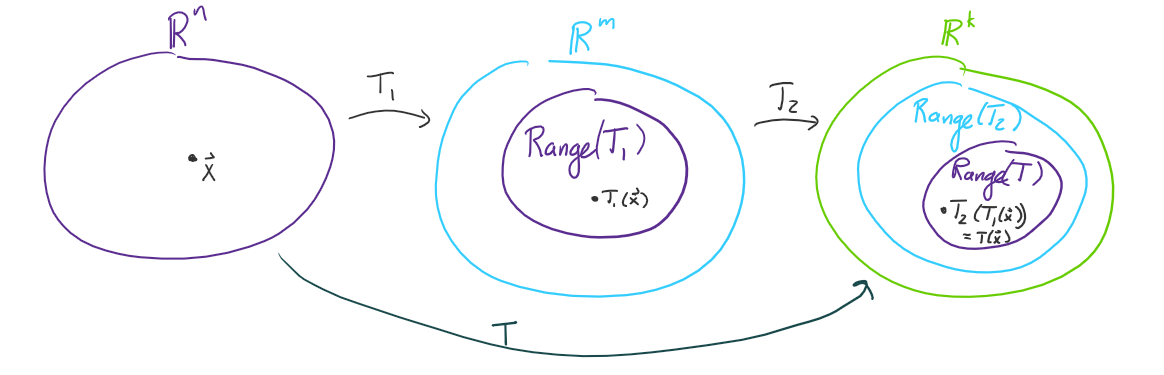
\includegraphics[width=.9\textwidth]{images/composition}
		\end{center}
	\end{defn}
\end{frame}
\begin{frame}{\fn}
	\begin{exercise}
		Let $T_1:\R^3\to\R^5$  be defined by $T_1(x,y,z)=(x,y,z,2x,y+z)$.
		
		Let $T_2:\R^5\to\R^2$ be defined by $T_2(x_1,x_2,x_3,x_4,x_5)=(x_1+x_2,x_3+x_4-x_5)$.
		
		Let $T=T_2\circ T_1$.  
		\begin{enumerate}[label=(\alph*)]
			\item What is the domain of $T$?  
			\item What is the codomain of $T$?
			\item Compute $T(1,0,0)$, $T(0,1,0)$, and $T(0,0,1)$.
		\end{enumerate}
	\end{exercise}
\end{frame}
\begin{frame}{\fn}
	\begin{statementblock}{Theorem 6.11}
		Let $T_1:\R^n\to \R^m$ and $T_2:\R^m\to \R^k$ be linear transformations with standard matrices $A_1$ and $A_2$, respectively.
		Then the composition $T:\R^n\to\R^k$ is also a linear transformation whose standard matrix is $A=A_2A_1$.
	\end{statementblock}
	\begin{exercise}
	Let $T_1:\R^3\to\R^5$  be defined by $T_1(x,y,z)=(x,y,z,2x,y+z)$.
	
	Let $T_2:\R^5\to\R^2$ be defined by $T_2(x_1,x_2,x_3,x_4,x_5)=(x_1+x_2,x_3+x_4-x_5)$.
	
	Let $T=T_2\circ T_1$.
	\begin{enumerate}[label=(\alph*)]
		\item Compute, via Theorem 6.10, the standard matrix $A_1$ of $T_1$, $A_2$ of $T_2$, and $A$ of $T$.
		\item Verify that $A=A_2A_1$.
	\end{enumerate}
	\end{exercise}
\end{frame}
\begin{frame}{\fn}
	\begin{block}{\textbf{Brain Break.}}
		Would you rather have a slice of Chicago style pizza, New York style pizza, or Italian style pizza?
		\vskip .25in
			
\includegraphics[height=.75in]{images/chicago_pizza}
			\hfill
			
\includegraphics[height=.75in]{images/new_york_pizza}
			\hfill
			\includegraphics[height=.75in]{images/italian_pizza}
		\vskip .25in
		I am a fan of an Italian margarita pizza fired in a brick oven.
	\end{block}
\end{frame}
\begin{frame}{\fn}
	\begin{exercise}
		Prove Theorem 6.11.  Particularly, prove the result stating that $T=T_2\circ T_1$ is a linear transformation.
		\begin{enumerate}[label=(\alph*)]
			\item Let $T_1:\R^n\to\R^m$ and $T_2:\R^m\to \R^k$ be linear transformations.
			\item Recall that in order to prove $T=T_2\circ T_1$ is a linear transformation, we need to show $T(\vec u+\vec v)=T(\vec u)+T(\vec v)$ and $T(c\vec u)=cT(\vec u)$.
			\item Using the definition of $T$, e.g.~$T(\vec u+\vec v)=T_2(T_1(\vec u+\vec v))$, prove the distributivity of $T$.
			\item Similarly prove the scalar factorization.
		\end{enumerate}
	\end{exercise}
\end{frame}
\begin{frame}{\fn}
	\begin{exercise}
		Consider the transformations $T_1:\R^3\to\R^2$ and $T_2:\R^2\to \R^3$ defined by
			\[T_1(x,y,z)=(x-y,x-z)\text{ and }T_2(x,y)=(3x,4y,0).\]
		\begin{enumerate}[label=(\alph*)]
			\item Find the standard matrices for $T_1$ and $T_2$.
			\item Use your answers to (a) to find the standard matrices of $T=T_2\circ T_1$ and of $T'=T_1\circ T_2$.
		\end{enumerate}
	\end{exercise}
\end{frame}
\begin{frame}{\fn}
	\begin{defn}
		If $T_1:\R^n\to\R^n$ and $T_2:\R^n\to \R^n$ are linear transformations such that for every $\vec v\in\R^n$, \[T_2\circ T_1(\vec v)=\vec v\text{ and }T_1\circ T_2(\vec v)=\vec v\]then $T_2$ is called the \emph{inverse} of $T_1$, and $T_1$ is said to be invertible.
	\end{defn}
	\begin{exercise}
		Let $T_1:\R^2\to\R^2$ and $T_2:\R^2\to\R^2$ be defined by 	
			\[T_1(x,y)=(x,x+y)\textup{ and }T_2(x,y)=(x,y-x)\]
		Show that $T_2$ is the inverse of $T_1$.
	\end{exercise}
\end{frame}
\begin{frame}{\fn}
	\begin{statementblock}{Theorem 6.12}
		Let $T:\R^n\to\R^n$ be a linear transformation with standard matrix $A$.  Then the following are equivalent.	
		\begin{enumerate}[label=\textbf{\arabic*}]
			\item $T$ is an invertible linear transformation.
			\item $T$ is an isomorphism.
			\item $A$ is an invertible matrix.
		\end{enumerate}
		Moreover, if $T$ is invertible, then the standard matrix for $T^{-1}$ is $A^{-1}$.
	\end{statementblock}
\end{frame}
\begin{frame}{\fn}
	\begin{exercise}
		Consider the linear transformation $T:\R^3\to\R^3$ defined by $T(x,y,z)=(3x-2y,x+y+2z,2x+y+z)$.  Determine whether $T$ is invertible.  If so, find its inverse:
			\begin{enumerate}[label=(\alph*)]
				\item Find the standard matrix, $A$, for $T$.
				\item Find the inverse of $A$.
				\item Then $T^{-1}(\vec v)=A^{-1}\vec v$.
				\item Write $T^{-1}$ in the form $T^{-1}(x,y,z)=(a,b,c)$ where $a,b$ and $c$ are linear functions of $x,y$ and $z$.
			\end{enumerate}
	\end{exercise}
\end{frame}
%\begin{frame}{\fn}
%	\begin{exercise}
%		Consider the linear transformation $T:\R^2\to\R^2$ defined by $T(x,y)=(x+y,3x+3y)$.  Determine whether $T$ is invertible.  If so, find its inverse.
%	\end{exercise}
%	\begin{exercise}
%	Consider the linear transformation $T:\R^4\to\R^4$ defined by $T(x,y,z,w)=(x-2y,y,z+w,z)$.  Determine whether $T$ is invertible.  If so, find its inverse.
%	\end{exercise}
%\end{frame}
%\begin{frame}{\fn}
%	\begin{exercise}
%		Consider the transformation $T:P_2\to P_2$ defined by $T(p(x))=xp'(x)$.  Similarly to Exercise 4, we can find a standard matrix for $T$ by encoding the polynomial $ax^2+bx+c$ as the vector $[p]=(a,b,c)$.  Use this encoding to find the standard matrix for $T$.  Is $T$ invertible?
%	\end{exercise}
%\end{frame}
%\begin{frame}{\fn}
%	\begin{exercise}
%		Consider the vector space $V$ that is all continuous functions of the form $a+b(x)+c(e^x)+d(xe^x)$.  Let $D:V\to V$ be the derivative transformation.  
%		
%		Encode elements of $V$ as vectors in $\R^4$ via \[[a+b(x)+c(e^x)+d(xe^x)] = \begin{bmatrix}a\\b\\c\\d\end{bmatrix}.\]
%		
%		\begin{enumerate}[label=(\alph*)]
%			\item Find the standard matrix for $D$ with respect to this correspondence.
%		
%			Recall that $D(1)=0$, $D(x)=1$, $D(e^x)=e^x$ and $D(xe^x)=e^x+xe^x$.
%			\item Use the standard matrix from part (a) to compute $D(2+4x-e^x+3xe^x)$.
%		\end{enumerate}
%		
%		
%	\end{exercise}
%\end{frame}
\end{document}

